\documentclass[10pt, xcolor=x11names, compress]{beamer}
\usetheme{progressbar}
%\usecolortheme[named=Purple4]{structure}
\progressbaroptions{headline=sections,titlepage=normal,frametitle=normal}

\setbeamertemplate{navigation symbols}{}

\usepackage{iwona} 

\usepackage{alltt}
\usepackage{amsmath,amsfonts, amssymb, amscd}
\usepackage{hyperref}
\usepackage{setspace}
\usepackage{wasysym}
\usepackage{ulem}

\usepackage{calc}
\usepackage[overlay,absolute]{textpos}
\TPGrid[5mm,5mm]{20}{20}



\renewcommand{\Re}{\operatorname{Re}}
\renewcommand{\Im}{\operatorname{Im}}
\newcommand{\debye}{\operatorname{debye}}

\newcommand{\chik}{$\chi(k)$}
\newcommand{\chir}{$|\tilde{\chi}(R)|$}


\newcommand{\file}[1]{{\color{Firebrick4}\texttt{`#1'}}}
\newcommand{\multiple}{{\color{Orange3}\textsl{multiple}}}


\newcommand{\atoms}  {{\color{DarkOrchid4}\textsc{atoms}}}
\newcommand{\feff}   {{\color{DarkOrchid4}\textsc{feff}}}
\newcommand{\ifeffit}{{\color{DarkOrchid4}\textsc{ifeffit}}}
\newcommand{\athena} {{\color{DarkOrchid4}\textsc{athena}}}
\newcommand{\artemis}{{\color{DarkOrchid4}\textsc{artemis}}}

\renewenvironment<>{center}
{\begin{actionenv}#1\begin{originalcenter}}
{\end{originalcenter}\end{actionenv}}

\definecolor{guessp}   {rgb}{0.64,0.00,0.64}
\newcommand{\guessp}   {{\color{guessp}guess}}
\definecolor{defp}     {rgb}{0.00,0.55,0.00}
\newcommand{\defp}     {{\color{defp}def}}
\definecolor{setp}     {rgb}{0,0,0}
\newcommand{\setp}     {{\color{setp}set}}
\definecolor{lguessp}  {rgb}{0.24,0.11,0.56}
\newcommand{\lguessp}  {{\color{lguessp}lguess}}
\definecolor{skipp}    {rgb}{0.70,0.70,0.70}
\newcommand{\skipp}    {{\color{skipp}skip}}
\definecolor{restrainp}{rgb}{0.80,0.61,0.11}
\newcommand{\restrainp}{{\color{restrainp}restrain}}
\definecolor{afterp}   {rgb}{0.29,0.44,0.55}
\newcommand{\afterp}   {{\color{afterp}after}}
\definecolor{penaltyp} {rgb}{0.55,0.35,0.17}
\newcommand{\penaltyp} {{\color{penaltyp}penalty}}
\definecolor{mergep}   {rgb}{0.93,0.00,0.00}
\newcommand{\mergep}   {{\color{mergep}merge}}


\newtheorem{conclusion}[theorem]{Conclusion}
\newtheorem{notethis}[theorem]{Note}

\newcommand{\eto}{EuTiO$_3$}
\newcommand{\pto}{PbTiO$_3$}
\newcommand{\pgt}{Pb$_{1-x}$Ge$_x$Te}
\newcommand{\lsco}{La$_{1-x}$Sr$_x$CuO$_4$}
\newcommand{\abc}{AgBr$_{1-x}$Cl$_x$}
\newcommand{\nicn}{$\big[$Ni(CN)$_4\big]$$^{2-}$}
\newcommand{\knicn}{K$_2$Ni(CN)$_4$}

% \newcommand{\GMS}{\mathbb{G}}
% \newcommand{\Gnot}{\mathsf{G^0}}
% \newcommand{\tmat}{\mathsf{t}}
% \newcommand{\boldr}{\boldsymbol{r}}

%% Time-stamp: <2011-10-26 17:01:33 bruce>
%%%%%%%%%%%%%%%%%%%%%%%%%%%%%%%%%%%%%%%%%%%%%%%%%%%%%%%%%%%%%%%%%%%%%%
%%%  Include file for
%%%    A Practical Introduction to Multiple Scattering Theory
%%%                            Copyright (C) 2004-2005, 2011 Bruce Ravel
%%%                            <bravel@anl.gov>
%%%                            http://feff.phys.washington.edu/~ravel
%%%%%%%%%%%%%%%%%%%%%%%%%%%%%%%%%%%%%%%%%%%%%%%%%%%%%%%%%%%%%%%%%%%%%%
%%
%% This work is licensed under the Creative Commons Attribution,
%% Share-Alike License. To view a copy of this license, visit
%% http://creativecommons.org/licenses/by-sa/2.5/ or send a letter to
%% Creative Commons, 559 Nathan Abbott Way, Stanford, California
%% 94305, USA.
%%
%%%%%%%%%%%%%%%%%%%%%%%%%%%%%%%%%%%%%%%%%%%%%%%%%%%%%%%%%%%%%%%%%%%%%%

%%% single scattering
\def  \SS {{
%  \begin{minipage}[h][3truecm][c]{4truecm}
  \begin{picture}(80,26)(0,0)
    \linethickness{1pt}
    \qbezier(8,13)(40,26)(72,13)
    \qbezier(8,13)(40,0)(72,13)
    {\color{red}
    \put(8,13){\circle*{9}}}
    {\color{Gold2}
    \put(72,13){\circle*{9}}}
  \end{picture}
%  \end{minipage}
}}

%%% double scattering
\def  \DS {{
  \begin{minipage}[h][2truecm][c]{3truecm}
  \begin{picture}(125,60)(0,0)
    \linethickness{1pt}
    \qbezier(12.5,20)(25,40)(62.5,50)
    \qbezier(62.5,50)(100,40)(112.5,20)
    \qbezier(12.5,20)(62.5,0)(112.5,20)
    {\color{red}
    \put(12.5,20){\circle*{13}}}
    {\color{blue}
    \put(59,50){\circle*{13}}
    \put(112.5,20){\circle*{13}}}
  \end{picture}
  \end{minipage}
}}

%%% triple scattering #1
\def  \TST {{
  \begin{minipage}[h][2truecm][c]{3truecm}
  \begin{picture}(125,60)(0,0)
    \linethickness{1pt}
    \qbezier(12.5,20)(25,40)(62.5,50)
    \qbezier(62.5,50)(100,40)(112.5,20)
    \qbezier(12.5,20)(50,30)(62.5,50)
    \qbezier(62.5,50)(75,30)(112.5,20)
    {\color{red}
    \put(12.5,20){\circle*{13}}}
    {\color{blue}
    \put(59,50){\circle*{13}}
    \put(112.5,20){\circle*{13}}}
  \end{picture}
  \end{minipage}
}}

%%% triple scattering #2
\def  \TSF {{
  \begin{minipage}[h][2truecm][c]{3truecm}
  \begin{picture}(125,60)(0,-20)
    \linethickness{1pt}
    \qbezier(12.5,20)(25,40)(62.5,50)
    \qbezier(62.5,50)(100,40)(112.5,20)
    \qbezier(62.5,-10)(100,0)(112.5,20)
    \qbezier(12.5,20)(25,0)(62.5,-10)
    {\color{red}
    \put(12.5,20){\circle*{13}}}
    {\color{blue}
    \put(59,50){\circle*{13}}
    \put(112.5,20){\circle*{13}}
    \put(59,-10){\circle*{13}}}
  \end{picture}
  \end{minipage}
}}

%% focussed DS
\def  \FDS {{
  \begin{picture}(80,26)(0,0)
    \linethickness{1pt}
    \qbezier(8,13)(20,26)(40,13)
    \qbezier(8,13)(40,0)(72,13)
    \qbezier(40,13)(56,26)(72,13)
    {\color{red}
    \put(8,13){\circle*{9}}}
    {\color{Gold2}
    \put(36,13){\circle*{9}}}
    {\color{Gold2}
    \put(68,13){\circle*{9}}}
  \end{picture}
}}

%% focussed TS
\def  \FTS {{
  \begin{picture}(80,26)(0,0)
    \linethickness{1pt}
    \qbezier(8,13)(20,26)(40,13)
    \qbezier(40,13)(56,26)(72,13)
    \qbezier(8,13)(20,0)(40,13)
    \qbezier(40,13)(56,0)(72,13)
    {\color{red}
    \put(8,13){\circle*{9}}}
    {\color{Gold2}
    \put(36,13){\circle*{9}}}
    {\color{Gold2}
    \put(68,13){\circle*{9}}}
  \end{picture}
}}

% %  \begin{minipage}[h][1truecm][c]{8truecm}
%   \begin{picture}(250,60)(0,0)
%     \linethickness{1pt}
%     \qbezier(12.5,20)(62.5,40)(125,20)
%     \qbezier(125,20)(187.5,40)(225.5,20)
%     \qbezier(12.5,20)(112.5,0)(225.5,20)
%     {\color{Firebrick4}
%     \put(12.5,20){\circle*{13}}}
%     {\color{blue}
%     \put(125,20){\circle*{13}}
%     \put(225.5,20){\circle*{13}}}
%   \end{picture}
% %  \end{minipage}

% %% focussed TS
% \def  \FTS {{
% %  \begin{minipage}[h][1truecm][c]{8truecm}
%   \begin{picture}(250,60)(0,0)
%     \linethickness{1pt}
%     \qbezier(12.5,20)(62.5,40)(125,20)
%     \qbezier(125,20)(187.5,40)(225.5,20)
%     \qbezier(12.5,20)(62.5,0)(125,20)
%     \qbezier(125,20)(187.5,0)(225.5,20)
%     {\color{Firebrick4}
%     \put(12.5,20){\circle*{13}}}
%     {\color{blue}
%     \put(125,20){\circle*{13}}
%     \put(225.5,20){\circle*{13}}}
%   \end{picture}
% %  \end{minipage}
% }}


%%% Local Variables:
%%% mode: latex
%%% TeX-master: t
%%% End:


\mode<presentation>

\title{A Practical Introduction to Multiple Scattering Theory}

\author{Bruce Ravel}
\institute[NIST]{Synchrotron Methods Group, Materials Measurement Science Division\\%
  Materials Measurement Laboratory\\%
  National Institute of Standards and Technology\\%
  \&\\%
  Local Contact, Beamline X23A2\\%
  National Synchrotron Light Source\\~}


\date[APS EXAFS 07]{2007 APS EXAFS Summer School\\July 23-27, 2007\\~}

\begin{document}
\maketitle

\begin{frame}
  \frametitle{Copyright}
  \tiny

  This document is copyright \copyright 2007-2010 Bruce Ravel.

  \begin{center}
    
\includegraphics[width=1.0cm]{images/somerights20}
  \end{center}

  This work is licensed under the Creative Commons
  Attribution-ShareAlike License.  To view a copy of this license,
  visit \href{http://creativecommons.org/licenses/by-sa/3.0/}
  {\color{Purple4}\texttt{http://creativecommons.org/licenses/by-sa/3.0/}}
  or send a letter to Creative Commons, 559 Nathan Abbott Way,
  Stanford, California 94305, USA.

  \begin{description}
  \item[You are free:] %
    \begin{itemize}
    \item \textbf{to Share} --- to copy, distribute, and transmit the work
    \item \textbf{to Remix} --- to adapt the work
    \end{itemize}
  \item[Under the following conditions:] %
    \begin{itemize}
    \item Attribution. You must attribute the work in the manner
      specified by the author or licensor (but not in any way that
      suggests that they endorse you or your use of the work).
    \item Share Alike. If you alter, transform, or build upon this
      work, you may distribute the resulting work only under the same,
      similar or a compatible license.
    \item Any of these conditions can be waived if you get permission
      from the author.
    \end{itemize}
  \end{description}
  \begin{itemize}
  \item For any reuse or distribution, you must make clear to others
    the license terms of this work. The best way to do this is with a
    link to the URL for this document.
  \item Any of the above conditions can be waived if you get
    permission from the copyright holder.
  \item Nothing in this license impairs or restricts the author's
    moral rights.
  \end{itemize}

  Your fair dealing and other rights are in no way affected by the
  above.  This is a human-readable summary of the Legal Code (the full
  license).


\end{frame}

%%% Local Variables:
%%% mode: latex
%%% TeX-master: "pimst2"
%%% End:

\begin{frame}
  \frametitle{Acknowledgements}
  Matt
\end{frame}

\section{Introduction}

\begin{frame}
  \frametitle{What I hope you take away from this talk}
  \begin{itemize}
  \item A broad outline of multiple scattering theory with enough
    background to talk with a theorist
  \item An understanding of how multiple scattering theory is used to
    interpret \textbf{XANES} spectra
  \item An understanding of how multiple scattering theory is used to
    analyze \textbf{EXAFS} spectra
  \item Some ideas about how to incorporate multiple scattering theory
    in your research
  \end{itemize}
\end{frame}

\begin{frame}
  \frametitle{This talk is about Feff}

  There are many approaches to spectroscopy theory out there,
  including multiplets, band structure, and finite difference methods.

  \bigskip

  \begin{exampleblock}{This talk is about Feff}
    \textsc{feff} is a real-space, multiple scattering code.
  \end{exampleblock}
  
  \bigskip

  \begin{itemize}
  \item A conceptual summary and simple physical interpretation of
    what ``real-space multiple scattering'' means.
  \item How RSMS is used to make XANES calculations.
  \item How RSMS is used in fitting EXAFS data.
  \end{itemize}
\end{frame}

\begin{frame}
  \frametitle{XAS Data}
  \begin{columns}<1->
    \begin{column}{0.35\linewidth}
      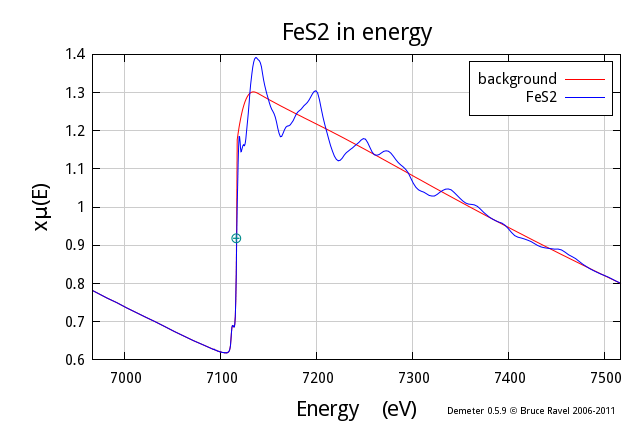
\includegraphics[width=\linewidth]{images/FeS2_mu.png}
    \end{column}
    \begin{column}{0.65\linewidth}
      We measure the {\color{Blue4}XAS data} and find the
      {\color{Red3}background function}
      \begin{equation}
        \mu(E) = \mu_0(E)\cdot\big(1+\chi(E)\big)
        \notag
      \end{equation}
    \end{column}
  \end{columns}
  \begin{columns}<2->
    \begin{column}{0.35\linewidth}
      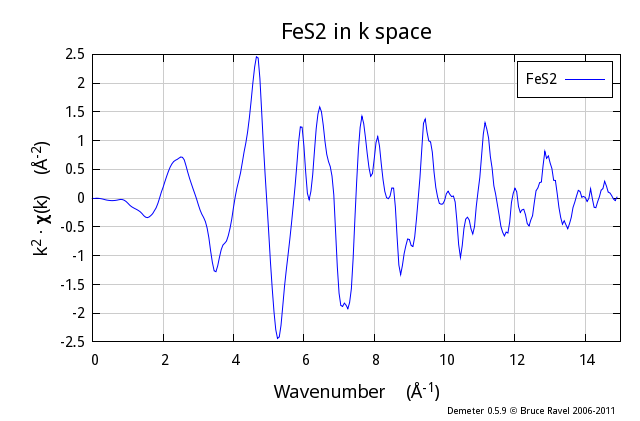
\includegraphics[width=\linewidth]{images/FeS2_chik.png}
    \end{column}
    \begin{column}{0.65\linewidth}
      We subtract the background, $\mu_0(E)$, to isolate the ``fine
      structure'' $\chi(k)$.  

      {\scriptsize (Remember, \alert{EXAFS} $\equiv$ \alert{E}xtended
        \alert{X}-ray \alert{A}bsorption \underline{\alert{F}ine
        \alert{S}tructure}.)}
    \end{column}
  \end{columns}
  \begin{columns}<3>
    \begin{column}{0.35\linewidth}
      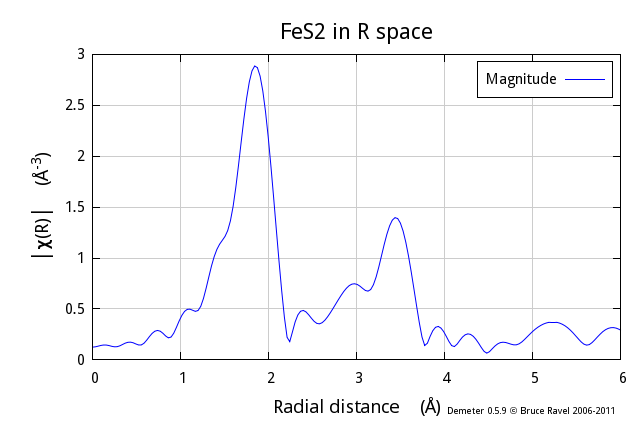
\includegraphics[width=\linewidth]{images/FeS2_chir.png}
    \end{column}
    \begin{column}{0.65\linewidth}
      We Fourier transform $\chi(k)$ and use \alert{multiple scattering
        theory} to understand the local structure.
    \end{column}
  \end{columns}
\end{frame}

\section{Real-space multiple scattering}

\begin{frame}
  \frametitle<1| handout:1>{A simple picture of X-ray absorption} 
  \frametitle<2| handout:2>{X-ray absorption in condensed matter}

  \begin{overlayarea}{\linewidth}{6ex}
    \only<1| handout:1>{An incident x-ray of energy $E$ is absorbed,
      destroying a core electron of binding energy $E_0$ and emitting
      a photo-electron with kinetic energy $(E-E_0)$. The core state
      is eventually filled, ejecting a fluorescent x-ray or an Auger
      electron.  }%
    \only<2| handout:2>{The ejected photo-electron can scatter from
      neighboring atoms. $R$ has some relationship to $\lambda$ and
      there is a phase shift associated with the scattering event.
      Thus the outgoing and scattered waves interfere.  }%
  \end{overlayarea}

  \vskip 20pt

  \begin{columns}[T]
    \begin{column}{0.5\linewidth}
      \only<1| handout:1>{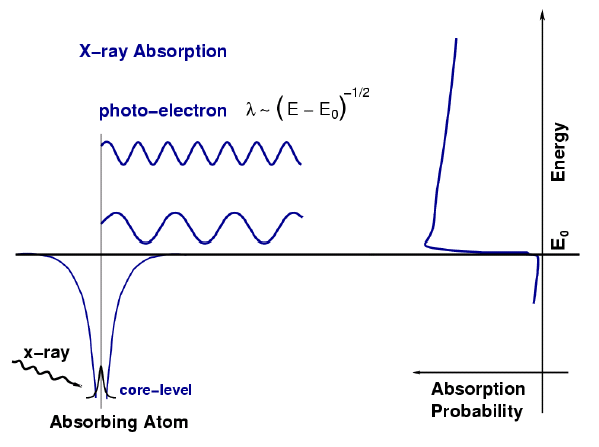
\includegraphics[width=\linewidth]{bare_atom.png}}
      \only<2| handout:2>{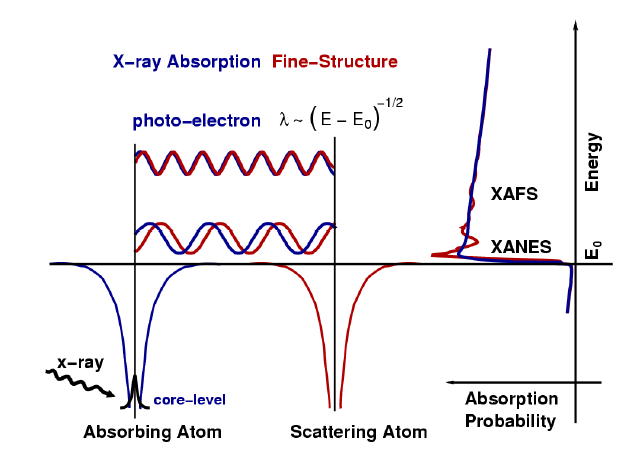
\includegraphics[width=\linewidth]{with_scattering.png}}
    \end{column}
    \begin{column}{0.5\linewidth}
      \begin{center}
        \only<1| handout:1>{
          An empty final state is required.\\
          {\alert{No available state, \\
              no absorption!}}\\
          When the incident x-ray energy is larger than the binding
          energy, there is a sharp increase in absorption.
        }
        \only<2| handout:2>{
          The scattering of the photo-electron wave function interferes
          with itself.\\[4ex]
          $\mu(E)$ depends on the density of states with energy
          $(E-E_0)$ at the absorbing atom.
        }
      \end{center}
    \end{column}
  \end{columns}

  \vskip 20pt

  \begin{overlayarea}{\linewidth}{3ex}
    \only<1| handout:1>{For an isolated atom, $\mu(E)$ has a sharp step at the
      core-level binding energy and is a smooth function of energy
      above the edge.}%
    \only<2| handout:2>{This interference \alert{at the absorbing atom} will vary
      with energy, causing the oscillations in $\mu(E)$.
    }%
  \end{overlayarea}
  \begin{bottomnote}[0.7][20] 
    Image from Matt Newville
  \end{bottomnote}
\end{frame}

\newcommand{\GMS}{\mathbb{G}}
\newcommand{\Gnot}{\mathsf{G^0}}
\newcommand{\tmat}{\mathsf{t}}
\newcommand{\boldr}{\boldsymbol{r}}

\begin{frame}[label=fgr]
  \frametitle{Computing X-ray Absorption from First Principles}
  \begin{columns}
    \begin{column}{0.75\linewidth}
      In XAS we measure the \alert{dipole mediated}$^\mathrm{[1]}$
      transition of an electron in a \alert{deep core}$^\mathrm{[2]}$
      state {\color{blue}$|i\rangle$} into an
      \alert{unoccupied}$^\mathrm{[3]}$ state
      {\color{Red4}$|f\rangle$}:

      \begin{columns}
        \begin{column}{0.15\linewidth}
          ~
        \end{column}
        \begin{column}{0.7\linewidth}
          \begin{block}{Fermi's Golden Rule}
            $\mu(E) \propto\> \sum\limits_f^{E_f>E_F}
            \big|{\color{Red4}\langle f|}
            {\color{blue}\hat{\epsilon}\cdot\mathbf{r}}
            {\color{blue}|i\rangle}\big|^2 \delta(E_f)$
          \end{block}
        \end{column}
        \begin{column}{0.15\linewidth}
          ~
        \end{column}
      \end{columns}

      \medskip

      Broadly speaking, there are two ways to solve this equation:
      \begin{enumerate}
      \item Accurately represent {\color{blue}$|i\rangle$}$^\mathrm{[4]}$  and
        {\color{Red4}$|f\rangle$}$^\mathrm{[5]}$, then evaluate
        the integral directly. This is the approach taken, for example, by
        molecular orbital theory.
      \item Use multiple scattering theory, AKA 
        propagator formalism$^\mathrm{[6]}$:\\
        {\footnotesize
        $\mu(E) \propto
        -\frac{1}{\pi} \Im {\color{blue}\langle \mathrm{i}
          |} \hat{\epsilon}^\ast \cdot \boldsymbol{r} \,
        {\color{Green4}\mathbb{G}(r,r';E)} \hat{\epsilon} \cdot \boldsymbol{r}' {\color{blue}|
          \mathrm{i} \rangle}
        \Theta(E-E_F)$.}
      \end{enumerate}      
    \end{column}
    \begin{column}{0.25\linewidth}
      \begin{enumerate}[1.]
        \scriptsize
      \item A photon interacts with an electron
      \item Typically a \textit{1s}, \textit{2s}, or \textit{2p} electron
      \item A bound or continuum state \textbf{not} already containing
        an electron
      \item Easy --- basic quantum mechanics
      \item Hard work, lots of computation
      \item {\color{Green4}$\GMS$} is also called a Green's function.
      \end{enumerate}
    \end{column}
  \end{columns}
\end{frame}

\begin{frame}
  \frametitle{Real Space Multiple Scattering}

  In multiple scattering theory, all the hard work is in computing
  the Green's function.

  \begin{description}
  \item[${\color{Green4}\GMS}$] the function that describes all
    possible ways for a photoelectron to interact with the
    surrounding atoms
  \item[$\Gnot$] the function that describes how an electron
    propagates between two points in space
  \item[$\tmat$] the function that describes how a photo-electron
    scatters from a neighboring atom
  \end{description}

  \begin{block}{Expanding the Green's function}
    ~\\[-6ex]
    \begin{align}
      {\color{Green4}\GMS} =& \big(1 - \Gnot \tmat\big)^{-1} \, \Gnot \tag{XANES}\\
      =& \Gnot + \Gnot\,\tmat\,\Gnot +
      \Gnot\,\tmat\,\Gnot\,\tmat\,\Gnot +
      \Gnot\,\tmat\,\Gnot\,\tmat\,\Gnot\,\tmat\,\Gnot + ... \tag{EXAFS}
    \end{align}
  \end{block}
\end{frame}

\begin{frame}{Scattering Paths}
  \textbf{Full multiple scattering (XANES):} Solving {\color{DarkOrchid4}
    ${\color{Green4}\GMS} = \big(1 - \Gnot \tmat\big)^{-1} \, \Gnot$}
  considers {\LARGE ALL} paths within some cluster of atoms:
  \begin{columns}[T]
    \begin{column}{0.33\linewidth}
      \begin{center}
        {\color{DarkOrchid4}single scattering path}\\
        {\color{blue}\SS}\\
        (2 legs)
      \end{center}
    \end{column}
    \begin{column}{0.33\linewidth}
      \begin{center}
        {\color{DarkOrchid4}double scattering path}\\
        {\color{blue}\FDS}\\
        (3 legs)
      \end{center}
    \end{column}
    \begin{column}{0.33\linewidth}
      \begin{center}
        {\color{DarkOrchid4}triple scattering path}\\
        {\color{blue}\FTS}\\
        (4 legs)
      \end{center}
    \end{column}
  \end{columns}

  \medskip

  \begin{exampleblock}{EXAFS path expansion}
    The clever thing about \textsc{feff} is that each term is further
    expanded as a sum of all paths of that order.

    \medskip

    {\color{DarkOrchid4}$\Gnot\,\tmat\,\Gnot$} is expanded as a sum of
    {\color{DarkOrchid4}single scattering} paths

    \medskip

    {\color{DarkOrchid4}$\Gnot\,\tmat\,\Gnot\,\tmat\,\Gnot$} is a sum
    of all {\color{DarkOrchid4}double scattering} paths

    \medskip

    and so on.
  \end{exampleblock}

\end{frame}



\newcommand{\FeLeft}{0.60\linewidth}
\newcommand{\FeRight}{0.38\linewidth}
\newcommand{\FeCluster}{0.65\linewidth}
\newcommand{\FePlot}{0.78\linewidth}

\begin{frame}
  \frametitle<1>{Iron metal: 1$^{\mathrm{st}}$ path, 1 shell }
  \frametitle<2>{Iron metal: 2$^{\mathrm{nd}}$ path, 2 shells }
  \frametitle<3>{Iron metal: 3$^{\mathrm{rd}}$ path, 1 shell }
  \frametitle<4>{Iron metal: 4$^{\mathrm{th}}$ path, 2 shells }
  \frametitle<5>{Iron metal: 5$^{\mathrm{th}}$ path, 3 shells }
  \frametitle<6>{Iron metal: 8$^{\mathrm{th}}$ path, 4 shells }

  \begin{columns}[T]
    \begin{column}{0.60\linewidth}
      \centering\includegraphics<1>[width=\FeCluster]{images/path1_diagram}
      \centering\includegraphics<2>[width=\FeCluster]{images/path2_diagram}
      \centering\includegraphics<3>[width=\FeCluster]{images/path3_diagram}
      \centering\includegraphics<4>[width=\FeCluster]{images/path4_diagram}
      \centering\includegraphics<5>[width=\FeCluster]{images/path5_diagram}
      \centering\includegraphics<6>[width=\FeCluster]{images/path8_diagram}
      \begin{enumerate}
      \item %
        \only<1>{The first path is much, but not all, of the first peak in {\chir}.}
        \only<2>{The second path overlaps the first in {\chir}.}
        \only<3>{This path contributes little to {\chir}.}
        \only<4>{This path contributes little to {\chir}.}
        \only<5>{This 3$^{\mathrm{rd}}$ shell SS path contributes most
          of the spectral weight to the second peak of {\chir}.}
        \only<6>{The 4$^{\mathrm{th}}$ shell SS path contributes to
          the third peak in {\chir}.}\\
        {\color{Firebrick3}Degeneracy = \only<1>{8}\only<2>{6}\only<3>{24}\only<4>{48}\only<5>{12}\only<6>{24}}
      \item %
        \only<1>{The first shell XANES calculation shows little of the
          structure.}
        \only<2>{The XANES calculation begins to show the structure of
          the spectrum.}
        \only<3>{The contribution from this path and all higher order
          paths scattering among these atoms is in the first shell
          XANES calculation.}
        \only<4>{The contribution from this path and all higher order
          paths scattering among these the first two shells is in the
          second shell XANES calculation.}
        \only<5>{The first peak after the edge in the XANES is
          sharpened considerably by the addition of this shell.}
        \only<6>{Including this shell in the XANES calculation broadens
          the peak above the edge somewhat.  It also introduces the
          second shoulder.}
      \end{enumerate}
    \end{column}
    \begin{column}{0.38\linewidth}
      \centering
      \includegraphics<1>[width=\FePlot]{images/path1}
      \includegraphics<2>[width=\FePlot]{images/path2}
      \includegraphics<3>[width=\FePlot]{images/path3}
      \includegraphics<4>[width=\FePlot]{images/path4}
      \includegraphics<5>[width=\FePlot]{images/path5}
      \includegraphics<6>[width=\FePlot]{images/path8}

      \centering\color{Green4}\texttt{`feff000{\only<1>{1}\only<2>{2}\only<3>{3}\only<4>{4}\only<5>{5}\only<6>{8}}.dat'}
      %\only<2>{\color{Green4}\texttt{`feff0002.dat'}}
      %\only<3>{\color{Green4}\texttt{`feff0003.dat'}}
      %\only<4>{\color{Green4}\texttt{`feff0004.dat'}}
      %\only<5>{\color{Green4}\texttt{`feff0005.dat'}}
      %\only<6>{\color{Green4}\texttt{`feff0008.dat'}}

      \bigskip

      \includegraphics<1>[width=\FePlot]{images/xanes_shell1}
      \includegraphics<2>[width=\FePlot]{images/xanes_shell2}
      \includegraphics<3>[width=\FePlot]{images/xanes_shell1}
      \includegraphics<4>[width=\FePlot]{images/xanes_shell2}
      \includegraphics<5>[width=\FePlot]{images/xanes_shell3}
      \includegraphics<6>[width=\FePlot]{images/xanes_shell4}

      \centering{\color{blue}XANES}

      \bigskip

      ~

      \bigskip

      ~

    \end{column}
  \end{columns}
\end{frame}



\begin{frame}
  \frametitle{Iron metal: 10$^{\mathrm{th}}$ path + MS, 5 shells}
  \begin{columns}[T]
    \begin{column}{0.05\linewidth}
      ~
    \end{column}
    \begin{column}{0.4\linewidth}
      \begin{center}
        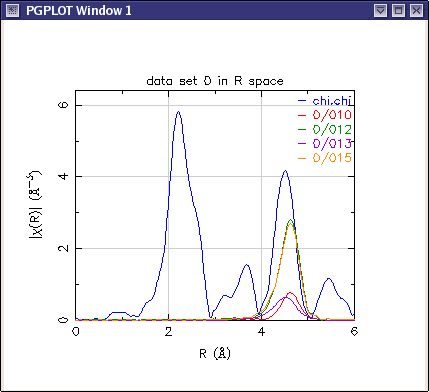
\includegraphics[width=0.75\linewidth]{images/path10}

        5$^{\mathrm{th}}$ shell EXAFS: Magnitude\\[2ex]

        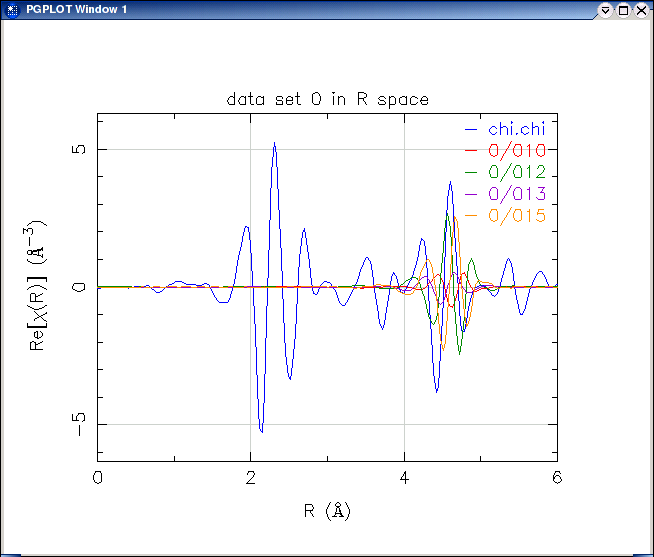
\includegraphics[width=0.75\linewidth]{images/path10_re}

        5$^{\mathrm{th}}$ shell EXAFS: Real part
      \end{center}
    \end{column}
    \begin{column}{0.1\linewidth}
      ~
    \end{column}
    \begin{column}{0.4\linewidth}
      \begin{block}{Convergence}
        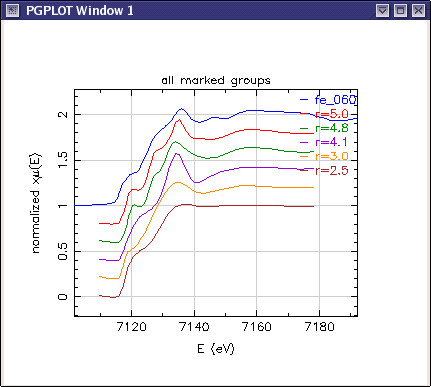
\includegraphics[width=\linewidth]{images/xanes_convergence}
      \end{block}
      There are several MS geometries with the same path length as the
      5$^{\mathrm{th}}$ shell SS path.  Some are \emph{bigger} than
      the SS path!
    \end{column}
    \begin{column}{0.05\linewidth}
      ~
    \end{column}
  \end{columns}
\end{frame}


% \section[XANES]{XANES Calculations}
% \subsection[Convergence of XANES]{\pto: Convergence of Full Multiple Scattering}

% 

\begin{frame}
  \frametitle{Test convergence in cluster size}
  \begin{tabular}[h]{cc}
    \begin{minipage}[h]{0.55\linewidth}
      \begin{center}
        %Below the plasmon resonance ($\sim40\,\mathrm{eV}$), 
        At low energy,%
        the photoelectron mean free path is quite large and it
        probes a large cluster of atoms.
        \begin{block}{The big question}
          How many atoms must be included in the cluster for a good
          \textsc{feff} calculation?
        \end{block}
        \begin{block}{The general answer}
          \centering{\color{red}Who knows?}
        \end{block}
        {\pto} has $c>a$ and the O and Ti atoms are displaced from
        sites of centrosymmetry.
      \end{center}
    \end{minipage} &
    \begin{minipage}[h]{0.43\linewidth}
      \begin{center}
        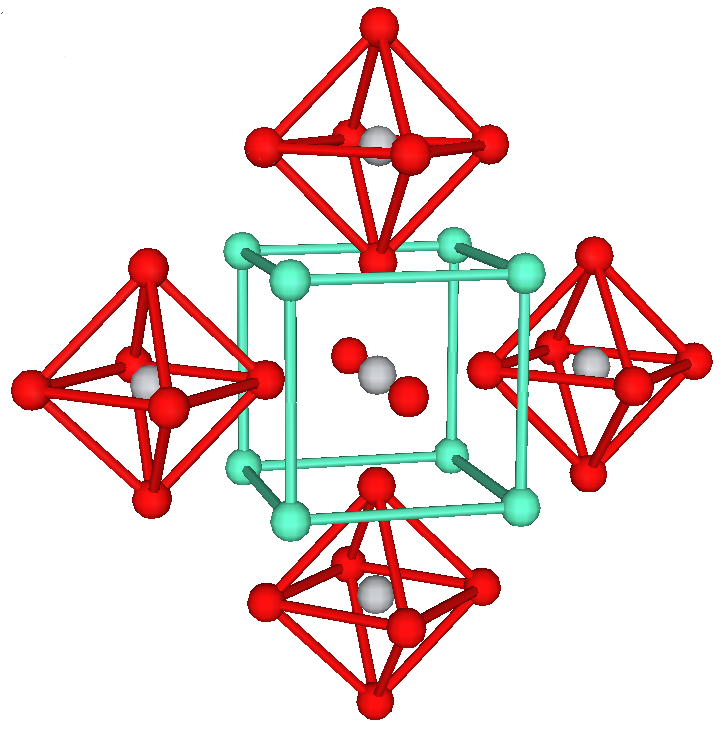
\includegraphics[height=0.95\linewidth]{images/PbTiO3/perovskite}

        \bigskip

        {\pto}: a tetragonally distorted perovskite\\
        {\color{SeaGreen2}$\bullet$} = Pb\quad
        {\color{Gray0}$\bullet$} = Ti\quad
        {\color{Red2}$\bullet$} = O
      \end{center}
    \end{minipage} \\
  \end{tabular}

\end{frame}

\begin{frame}
  \frametitle<1>{First coordination shell of \pto}
  \frametitle<2>{Second coordination shell of \pto}
  \frametitle<3>{Third coordination shell of \pto}
  \frametitle<4>{Fourth coordination shell of \pto}
  \frametitle<5>{Fifth coordination shell of \pto}
  \frametitle<6>{Sixth coordination shell of \pto}

  \setbeamercovered{transparent={50}}
  \begin{columns}[c]
    \begin{column}[c]{0.48\linewidth}
      \includegraphics<1>[width=0.85\linewidth]{images/PbTiO3/shell1}
      \includegraphics<2>[width=0.85\linewidth]{images/PbTiO3/shell2}
      \includegraphics<3>[width=0.85\linewidth]{images/PbTiO3/shell3}
      \includegraphics<4>[width=0.85\linewidth]{images/PbTiO3/shell4}
      \includegraphics<5>[width=0.85\linewidth]{images/PbTiO3/shell5}
      \includegraphics<6>[width=0.85\linewidth]{images/PbTiO3/shell6}
    \end{column}
    \begin{column}[c]{0.48\linewidth}
      \begin{enumerate}
      \item<1-| alert@1> \texttt{O:~~~}R=2.40\AA, 7 atoms
      \item<2-| alert@2| uncover@2-> \texttt{Pb:~~}R=3.60\AA, 15 atoms
      \item<3-| alert@3| uncover@3-> \texttt{Ti:~~}R=4.20\AA, 21 atoms
      \item<4-| alert@4| uncover@4-> \texttt{O:~~~}R=5.00\AA, 45 atoms
      \item<5-| alert@5| uncover@5-> \texttt{Ti:~~}R=5.71\AA, 57 atoms
      \item<6-| alert@6| uncover@6-> \texttt{O:~~~}R=6.30\AA, 86 atoms
      \end{enumerate}
    \end{column}
  \end{columns}

  \bigskip

  \begin{block}{Comment}
    \begin{minipage}[h][10ex][t]{1.0\linewidth}
      \only<1>{We see some indication of the structure just above the
        Fermi energy, but not much else.  Note that the memory
        requirement of the calculation goes as the square of the matrix
        size and the time goes as its cube!}%%
      \only<2>{The XANES structure begins to take shape, but all the
        features are broad.}%%
      \only<3>{Very little changes by adding the 3$^{\mathrm{rd}}$ shell
        Ti atoms!}%%
      \only<4>{Adding an oxygen shell causes the features to become much
        more distinct. Low Z elements have strong scattering at low k.
        High Z elements have strong scattering at high k.}%%
      \only<5>{Again, adding a metal shell does little for the
        spectrum.}%%
      \only<6>{Once again, adding an oxygen shell causes the features to
        become much more distinct. Low Z elements have a strong effect
        on the XANES.  Is the calculation converged?  Probably not.
        Large clusters are required!}%%
    \end{minipage}
  \end{block}
\end{frame}

\begin{frame}
  \frametitle{Scattering amplitude as a function of Z}
  PbTiO$_3$ has three very different elements:
  \begin{description}[Transition metal]
  \item[Low Z] Large at low $k$, tails off quickly
  \item[Transition metal] Large at intermediate $k$, tails off slowly
  \item[Heavy metal] Always there, but with a Ramsauer-Townsend minimum
  \end{description}

  \medskip

  \begin{columns}
    \begin{column}{0.6\linewidth}
      \centering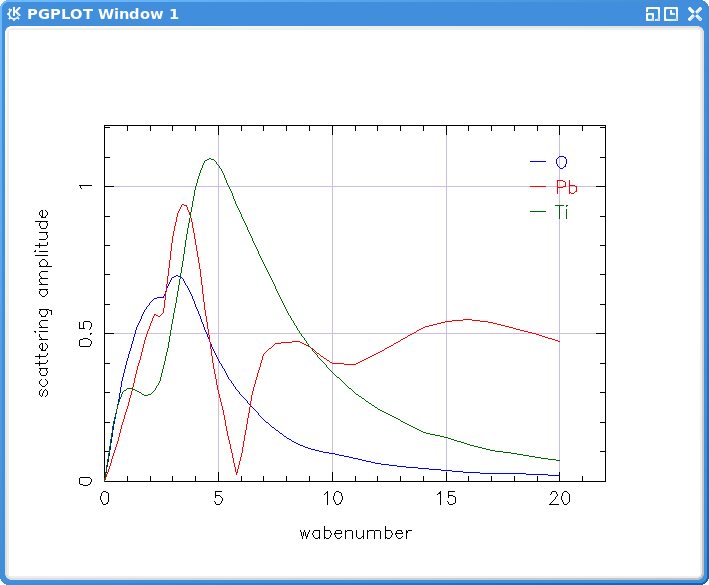
\includegraphics[width=0.85\linewidth]{images/PbTiO3/fofk}
    \end{column}
    %%
    \begin{column}{0.4\linewidth}
      \begin{block}{XANES and EXAFS}
        We can understand both the behavior of the XANES calculations
        and what we observe in EXAFS data.
    \end{block}
    \end{column}
  \end{columns}
\end{frame}

\begin{frame}
  \frametitle{Linear dichroism in \pto}
  \begin{columns}
    \begin{column}{0.48\linewidth}
      \begin{block}{$\overline{ab}$ plane}
        \centering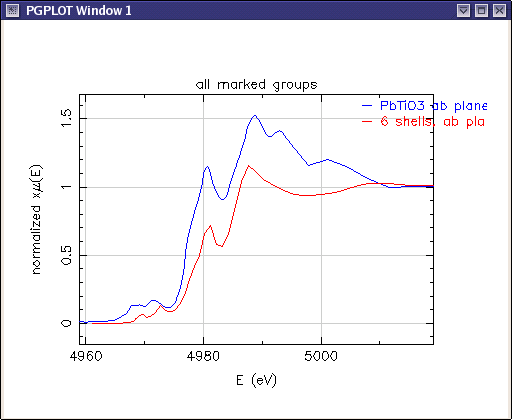
\includegraphics[width=0.85\linewidth]{images/PbTiO3/ab}
      \end{block}
    \end{column}
    \begin{column}{0.48\linewidth}
      \begin{block}{$\hat{c}$ axis}
        \centering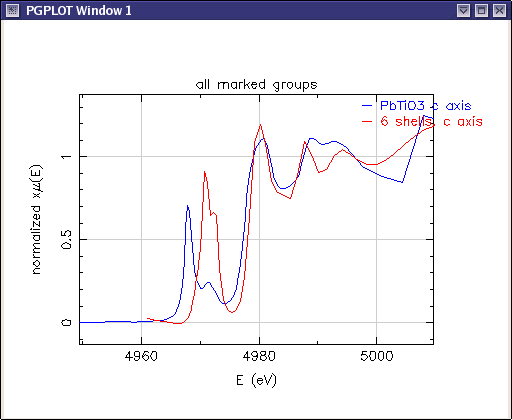
\includegraphics[width=0.85\linewidth]{images/PbTiO3/c}
      \end{block}
    \end{column}
  \end{columns}

  \bigskip

  \begin{center}
    Polarization can be included directly in the XANES calculation and
    shows the correct behavior compared to the data.
  \end{center}
\end{frame}

%%% Local Variables:
%%% mode: latex
%%% TeX-master: t
%%% End:

% \subsection[Interesting XANES Problems]{Solving interesting XANES problems}
% 
\begin{frame}
  \frametitle{Making useful XANES calculations}

  The challenge to using \textsc{feff}8 \textit{well} is that you need
  to provide a list of atomic coordinates.  But if you already know
  where the atoms are, you probably don't need to calculate the XANES.

  \bigskip

  In this section, we will briefly discuss how to handle

  \begin{itemize}
  \item Vacancies and substitutions
  \item Structural distortions
  \end{itemize}

  We will also discuss
  \begin{itemize}
  \item \textsc{feff}'s concept of computing {\color{Blue4}self
      consistent potentials}
  \item {\color{Blue4}Fitting} XANES spectra as implemented in
    \textsc{mxan} and \textsc{FitIt}.
  \end{itemize}
\end{frame}

\begin{frame}
  \frametitle{Vacancies and substitutions}
  \begin{itemize}
  \item In \textsc{feff}, a point in space is occupied by {\color{Blue4}one
      or zero} atoms and may not be partially vacant or fractionally
    occupied.
  \item These effects cannot be computed by a \alert{single}
    \textsc{feff} calculation.
  \item The most successful strategy is to make multiple calculations,
    randomly introducing substitutions or vacancies.
  \item Sum these calculations progressively until the average is
    converged.
  \item Convergence will probably happen within 10 or 20 calculations.
  \end{itemize}
\end{frame}

\begin{frame}
  \frametitle{Structural distortion}
  \begin{columns}
    \begin{column}{5cm}
      \centering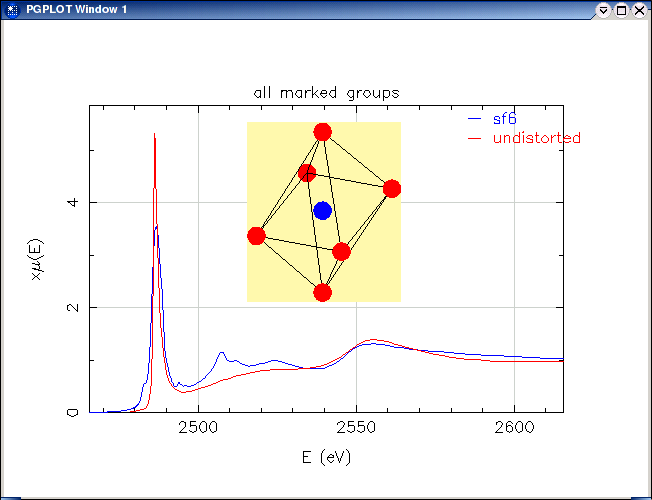
\includegraphics[width=0.9\linewidth]{images/SF6/sf6_undistorted}

      \centering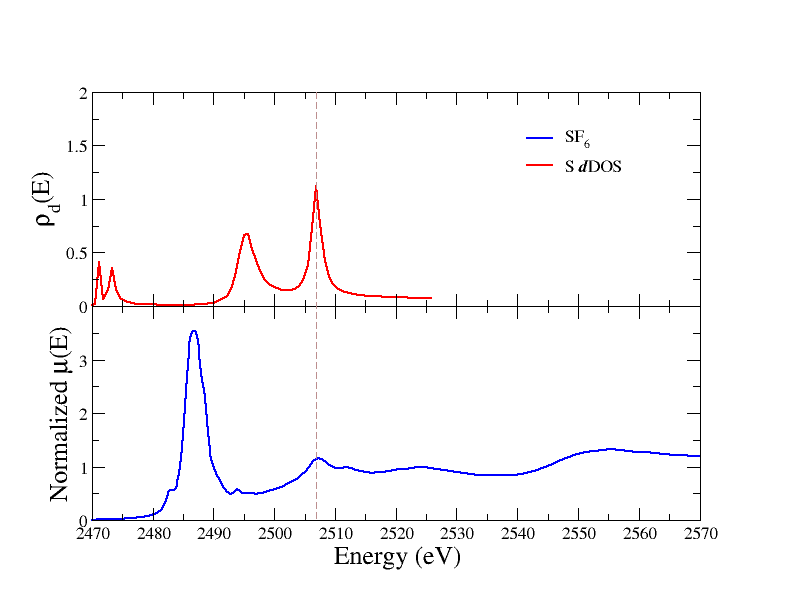
\includegraphics[width=0.9\linewidth]{images/SF6/ddos}
    \end{column}
    \begin{column}{6cm}
      SF$_6$ is an octahedral complex with nominal bond length of
      1.54\,\AA.  A distortion will mix \textit{p} and \textit{d}
      character in the final state with the peak near 2507\,eV in the
      \textit{d}DOS contributing spectrum.
      \begin{itemize}
      \item Thermal: $\langle R_{S,F_x} - R_{S,F_{-x}}\rangle \ne 0$
      \item Jahn-Teller
      \end{itemize}

      \medskip

      \centering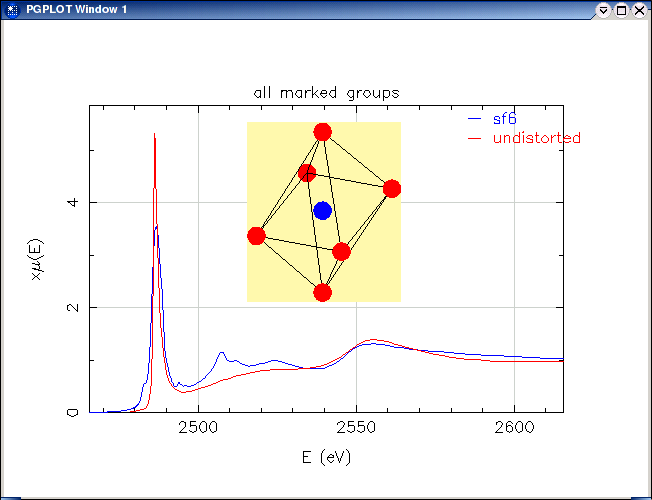
\includegraphics[width=0.86\linewidth]{images/SF6/sf6_undistorted}
    \end{column}
  \end{columns}
\end{frame}

\begin{frame}
  \frametitle{Self consistent potentials}

  \textsc{feff} starts with the potentials of the free atoms,
  $\rho_0(E)$.  It loops through the following calculations until
  the $\rho(E)$ functions stop changing.
  {\color{Blue4}
    \begin{equation*}
      \rho_\ell(E) = \rho_{0,\ell}(E)  \big(1 + \chi_\ell(E)\big)
      \qquad \ell \in \{0, 1, 2, 3, \cdots\}
    \end{equation*}
    }

  \begin{block}{Self consistency loop}
    \begin{equation*}
      \begin{CD}
        \rho_0(E) @>>> F(E),\Phi(E) @>>> \chi(E) \\
        && @AAA @VVV \\
        && \mathrm{converged?} @<<< \rho(E)
      \end{CD}
    \end{equation*}
  \end{block}

  \begin{center}
    At the end, $\rho(E)$ is integrated in energy.  The Fermi energy
    is where the integral equals the total number of valence electrons
    among the original free atoms in the cluster.  This integral also
    determines charge transfer.
  \end{center}
\end{frame}

\begin{frame}
  \frametitle{Fitting XANES spectra: Direct calculation}

  Compute XANES as a multivariate function of a large parameter space:
  \begin{definition}[Computed absorption]
    \centering$\mu(E,x_i,\alpha_j,\beta_k)$
  \end{definition}

  \begin{description}
    \item[$x_i$] the positions of all atoms in the cluster
    \item[$\alpha_j$]  parameters of the potentials model (muffin
      tin radii, loss terms, the Fermi energy, etc)
    \item[$\beta_k$] empirical parameters (broadening, $E_0$, offset
      function, etc)
  \end{description}


  \begin{block}{Fitting loop}
    \begin{equation*}
      \begin{CD}
        \mu_{\mathrm{init}}(E, x_i, \alpha_j, \beta_k) @>>>
        \mathrm{compare~to~data} @>>> \mathrm{adjust}~ x_i, \alpha_j, \beta_k \\
        && @AAA @VVV \\
        && \mu_{\mathrm{refined}}(E, x_i, \alpha_j, \beta_k) @<<< \mathrm{converged?}
      \end{CD}
    \end{equation*}
  \end{block}

  In the \textsc{feff} world, this is an open problem.  But see, for
  example, MXAN by M.\ Benfatto et al. PRB \textbf{65} (2002) 174205.
\end{frame}

\begin{frame}
  \frametitle{Fitting XANES spectra: multidimensional interpolation approximation}

  \begin{itemize}
  \item Another approach to the fitting XANES data is to precompute
    an adequate grid in the parameters $x_i$, $\alpha_j$, and
    $\beta_k$ and to place the data within that grid by
    multidimensional interpolation.
  \item This approach is quick after the initial computational expense.
  \item This has been implemented as the program \textsc{FitIt} by
    Grigory Smolentsev and Alexander V. Soldatov.  See
    \href{http://xafs.org/Software/FitIt}{\color{Purple4}\texttt{http://xafs.org/Software/FitIt}}
  \end{itemize}
\end{frame}

%%% Local Variables:
%%% mode: latex
%%% TeX-master: "pimst2"
%%% End:


%%\section[EXAFS]{Using Multiple Scattering in EXAFS}

\section{EXAFS equation}

%\againframe{fgr}

\begin{frame}
  \frametitle{Fermi's Golden Rule revisited}
  The absorption is the dipole mediated transition from the initial
  state of the deep-core electron to its final state:
  \begin{equation}
    \mu(E) \sim \big|\langle f| \mathcal{H}|i\rangle\big|^2
    \notag
  \end{equation}
  \begin{description}
  \item[The initial state $|i\rangle$] This is the deep core, atomic
    state which is unaffected by the surroundings
  \item[The excitation $\mathcal{H}$] The dipole operator, i.e.\ the
    incident photon
  \item[The final state $|f\rangle$] This high-lying or continuum
    state \alert{is} affected by the surroundings
  \end{description}
  \begin{block}{Consider $|f\rangle = |f_0+\Delta f\rangle$}
    \begin{itemize}
    \item $|f_0\rangle$ is the final state in the presence of the
      surrounding atoms but \alert{without} any scattering of the
      photoelectron
    \item $\Delta f$is the purturbation to the final state cause by
      the scattering of the photoelectron from the surrounding atoms
    \end{itemize}
  \end{block}
  \begin{textblock*}{0.6\linewidth}(0pt,19\TPVertModule)%
    \tiny%
    The discussion on the following 8 pages is inspired by Matt
    Newville's at
    \href{http://xafs.org/Tutorials?action=AttachFile&do=view&target=Newville_Intro.pdf}
    {\color{Blue4}\texttt{http://xafs.org/Tutorials?action=AttachFile\&do=view\&target=Newville\_Intro.pdf}}
  \end{textblock*}
\end{frame}


\begin{frame}
  \frametitle{The fine structure}
  With $|f\rangle = |f_0+\Delta f\rangle$
  \begin{align}
    \mu(E) \sim&\, \big|\langle \alert{f}| \mathcal{H}|i\rangle\big|^2
    \notag\\
    \sim&\, \big|\langle \alert{f_0}| \mathcal{H}|i\rangle\big|^2
    \big[
    1 + A(E)
    \big|\langle \alert{\Delta f}| \mathcal{H}|i\rangle\big|
    + C.C.
    \big]\notag\\
    \intertext{Remember that}
    \mu(E) =&\, \mu_0(E) \cdot (1+\chi(E))\notag\\
    \intertext{Therefore}
    \chi(E) \sim&\,\Big(\big|\langle \alert{\Delta f}|
    \mathcal{H}|i\rangle\big| + C.C.\Big)\notag
  \end{align}

  \begin{conclusion}
    The XAS fine structure, $\chi(E)$, is caused by the scattering from
    the neighboring atoms.
  \end{conclusion}

  \begin{textblock*}{0.6\linewidth}(0pt,19.25\TPVertModule)%
    \tiny%
    $A(E)$ contains a bunch of stuff having nothing to do with the
    scattering. $A(E) = \langle
      i|\mathcal{H}|\alert{f_0}\rangle^\ast / \big|\langle
      \alert{f_0}| \mathcal{H}|i\rangle\big|^2$
  \end{textblock*}
\end{frame}

\begin{frame}
  \frametitle{Heuristic derivation of the EXAFS equation}
  \begin{columns}
    \begin{column}{0.5\linewidth}
      The photoelectron:
      \begin{itemize}
      \item propagates as a spherical wave from absorber to scatterer
      \item scatters from the neighbor
      \item propagates as a spherical wave from scatterer to absorber
      \end{itemize}
    \end{column}
    \begin{column}{0.5\linewidth}
      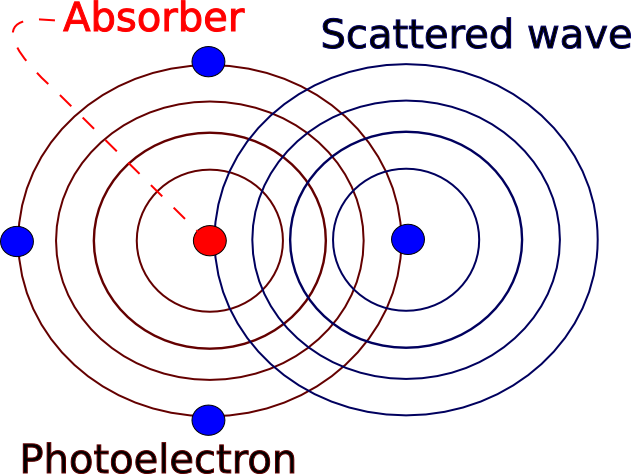
\includegraphics[width=\linewidth]{images/circles.png}
    \end{column}
  \end{columns}
  
  \bigskip

  Energy and photoelectron wavenumber are related by
  \begin{equation}
    k = \sqrt{2m_e(E-E_0)/\hbar^2} \simeq \alert{\sqrt{(E-E_0)/3.81}}\notag
  \end{equation}

  So, in terms of $k$
  \begin{equation}
    \chi(k) \sim \frac{e^{ikr}}{kr} \cdot
    2kF(k)e^{\phi(k)} \cdot
    \frac{e^{ikr}}{kr} + C.C.
    \notag
  \end{equation}
\end{frame}

\begin{frame}
  \frametitle{The EXAFS equation in its simplest form}
  We can now simplify the equation to
  \begin{equation}
    \chi(k) \sim \frac{F(k)}{2kR^2}\sin\big(2kR+\phi(k)\big)
    \notag
  \end{equation}
  This describes the signal from a single atom at a distance $R$.

  \medskip

  If we consider the contribution from $N$ atoms at distance $R$
  (i.e.\ a ``shell'' of atoms):
  \begin{equation}
    \chi(k) \sim \frac{NF(k)}{2kR^2}\sin\big(2kR+\phi(k)\big)
    \notag
  \end{equation}
  On the following pages, we consider
  \begin{enumerate}
  \item the shapes of $F(k)$ and $\phi(k)$
  \item the amplitude reduction term $S_0^2$
  \item the mean free path term $\lambda$
  \item disorder via the mean square displacement term $\sigma^2$
  \end{enumerate}
\end{frame}

\begin{frame}
  \frametitle{The complex photoelectron scattering factor}
  
\end{frame}

\begin{frame}
  \frametitle{The amplitude reduction factor}

  When the core electron is ejected from it's deep-core state, the
  remaining electrons relax:
  \begin{equation}
    S_0^2 = \big|\langle \Phi_f^{N-1}  | \Phi_i^{N-1}  \rangle
    \big|^2    \notag
  \end{equation}
  where $|\Phi^{N-1}\rangle$ is the state of all remaining electrons
  before ($i$) or after ($f$) the excitation.
  \begin{equation}
    \chi(k) \sim \frac{N\alert{S_0^2}F(k)}{2kR^2}\sin\big(2kR+\phi(k)\big)
    \notag
  \end{equation}
  In practice, $0.7\lesssim S_0^2<1.0$, but note that $N$ and $S_0^2$
  are completely correlated!
  \begin{textblock*}{0.6\linewidth}(0pt,19.25\TPVertModule)%
    \tiny%
    G.G.\ Li, F.\ Bridges, \& C.H.\ Booth, Phys. Rev. B \textbf{52}
    (1995) 6332--6348
    \href{http://dx.doi.org/10.1103/PhysRevB.52.6332}
    {\color{Blue4}\texttt{DOI:10.1103/PhysRevB.52.6332}}
  \end{textblock*}
\end{frame}

\begin{frame}
  \frametitle{The mean free path}
  The photoelecton may scatter \textit{inelastically} and fail to
  ``return'' to the absorber (loose coherence with the core-hole).

  \medskip

  \begin{columns}
    \begin{column}{0.5\linewidth}
      We consider this by replacing the photoelecton spherical wave
      with a damped spherical wave:
      $\frac{e^{ikr}e^{-r/\lambda(k)}}{kr}$

      \medskip

      Here is {\feff}'s calculation of the mean free path in copper
      metal.
    \end{column}
    \begin{column}{0.5\linewidth}
      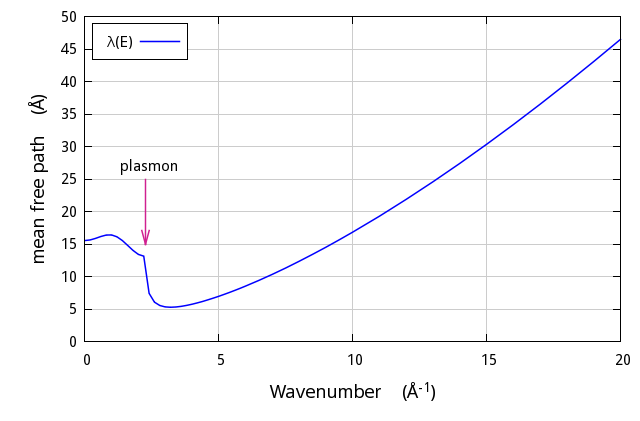
\includegraphics[width=\linewidth]{images/mfp.png}
    \end{column}
  \end{columns}
  \begin{equation}
    \chi(k) \sim \frac{NS_0^2F(k)}{2kR^2}\sin\big(2kR+\phi(k)\big)
    \alert{e^{-2R/\lambda(k)}}
    \notag
  \end{equation}
  \begin{notethis}
    $\frac{e^{-2R/\lambda(k)}}{R^2}$ is what makes EXAFS a \alert{local}
    structure probe.
  \end{notethis}
\end{frame}

\begin{frame}
  \frametitle{The mean square displacement (disorder)}
  Even in a highly ordered crystal -- like an FCC metal -- the atoms
  are never actually on their lattice positions.  \textit{Thermal
    motion} (i.e.\ phonons) distribute atoms around their nominal
  positions such that
  \begin{equation}
    \sigma_{i,j}^2 = \langle r_{i,j}-\overline{r_{i,j}} \rangle^2 > 0
    \notag
  \end{equation}
  This behaves some like the crystallographic Debye-Waller factor:
  \begin{exampleblock}{The standard EXAFS equation}
    \begin{equation}
      \chi(k) = \frac{NS_0^2F(k)}{2kR^2}\sin\big(2kR+\phi(k)\big)
      \alert{e^{-2k^2\sigma^2}}e^{-2r/\lambda(k)}
      \notag
    \end{equation}
  \end{exampleblock}

  \begin{textblock*}{0.8\linewidth}(0pt,17.5\TPVertModule)%
    {\scriptsize
      One can also consider higher moments of the distribution,
      $\sigma^n = \langle r_{i,j}-\overline{r_{i,j}} \rangle^n$.  See
    }\\
    {\tiny%
      G.\ Bunker, Nucl.\ Inst.\ Methods \textbf{207}:3 (1983) pp.\
      437--444,
      \href{http://dx.doi.org/10.1016/0167-5087(83)90655-5}
      {\color{Blue4}\texttt{DOI:10.1016/0167-5087(83)90655-5}}
    }
  \end{textblock*}
\end{frame}

\begin{frame}
  \frametitle{Multiple scattering paths}
  The magic of {\feff} is that it expresses the effect of multiple
  scattering events entirely in $F(k)$ and $\phi(k)$:
  \begin{equation}
    \chi(k) = \frac{NS_0^2\alert{F_{eff}(k)}}{2kR^2}
    \sin\big(2kR+\alert{\phi_{eff}(k)}\big)
    e^{-2k^2\sigma^2}e^{-2r/\lambda(k)}
    \notag
  \end{equation}
  That's the same equation!

  \begin{textblock*}{0.6\linewidth}(0pt,19.5\TPVertModule)%
    \tiny%
    S.I.\ Zabinsky et al, Phys. Rev. B \textbf{52} (1995) 2995--3009\\
    \href{http://dx.doi.org/10.1103/PhysRevB.52.2995}
    {\color{Blue4}\texttt{DOI:10.1103/PhysRevB.52.2995}}    
  \end{textblock*}
\end{frame}

\section[EXAFS]{Using FEFF to Solve EXAFS Problems}

\begin{frame}[fragile]
  \frametitle<1>{A Feff6 input file}
  \frametitle<2>{A Feff8 input file}
  \begin{columns}[T]
    \begin{column}{0.44\linewidth}
      Here is an example of a \textsc{feff}\only<1>6\only<2>8 input file:

      \vspace*{\stretch{1}}

      \begin{onlyenv}<1>
        \begin{block}{}
          \begin{alltt}
            \tiny
 {\color{Green4}TITLE Cobalt sulfide  CoS\_2}

 {\color{Purple2}HOLE} 1 1.0 {\color{Blue4}*  Co K edge (7709.0 eV)

 *         mphase,mpath,mfeff,mchi}
 {\color{SteelBlue2}CONTROL}   1      1     1     1
 {\color{SteelBlue2}PRINT}     1      0     0     0

 {\color{Purple2}RMAX}        6.0


 {\color{Brown4}POTENTIALS}
 {\color{Blue4}*    ipot   Z  element}
        0   27   Co
        1   27   Co
        2   16   S

                  {\color{Blue4}* continued ------>}
          \end{alltt}
        \end{block}
      \end{onlyenv}
      \begin{onlyenv}<2>
        \begin{block}{}
          \begin{alltt}
            \tiny
 {\color{Green4}TITLE Cobalt sulfide  CoS\_2}
 {\color{Purple2}EDGE} K
 {\color{Purple2}S02}  1.0

 {\color{Blue4} *    pot    xsph  fms   paths genfmt ff2chi}
 {\color{SteelBlue2}CONTROL}   1      1     1     1     1     1
 {\color{SteelBlue2}PRINT}     1      0     0     0     0     0

 {\color{Purple2}EXCHANGE}   0
 {\color{Purple2}SCF}        4.0
 {\color{Purple2}XANES}      4.0
 {\color{Purple2}FMS}        5.09694  0
 {\color{Purple2}LDOS}      -30   20     0.1
 {\color{Purple2}RPATH}      0.1
 {\color{Blue4}*EXAFS     20}

 {\color{Brown4}POTENTIALS}
 {\color{Blue4}*   ipot  Z  element  l\_scmt  l\_fms  stoi.}
        0   27   Co       2       2       0
        1   27   Co       2       2       4
        2   16   S        2       2       8
                          {\color{Blue4}* continued ------>}
          \end{alltt}
        \end{block}
      \end{onlyenv}
     \end{column}
     %%
     \begin{column}{0.54\linewidth}
      \begin{block}{}
         \begin{alltt}
         \tiny
  {\color{Brown4}ATOMS}   {\color{Blue4}* this list contains 71 atoms
  *   x          y          z     ipot  tag     distance}
     0.00000    0.00000    0.00000  0  Co1     0.00000
     2.14845    0.61305    0.61305  2  S1\_1    2.31678
     0.61305   -2.14845    0.61305  2  S1\_1    2.31678
    -0.61305    0.61305    2.14845  2  S1\_1    2.31678
    -0.61305    2.14845   -0.61305  2  S1\_1    2.31678
    -2.14845   -0.61305   -0.61305  2  S1\_1    2.31678
     0.61305   -0.61305   -2.14845  2  S1\_1    2.31678
    -3.37455    0.61305    0.61305  2  S1\_2    3.48415
     0.61305    3.37455    0.61305  2  S1\_2    3.48415
     0.61305   -0.61305    3.37455  2  S1\_2    3.48415
     3.37455   -0.61305   -0.61305  2  S1\_2    3.48415
    -0.61305   -3.37455   -0.61305  2  S1\_2    3.48415
    -0.61305    0.61305   -3.37455  2  S1\_2    3.48415
    -2.14845   -2.14845    2.14845  2  S1\_3    3.72122
     2.14845    2.14845   -2.14845  2  S1\_3    3.72122
     2.76150    2.76150    0.00000  1  Co1\_1   3.90535
    -2.76150    2.76150    0.00000  1  Co1\_1   3.90535
     2.76150   -2.76150    0.00000  1  Co1\_1   3.90535
    -2.76150   -2.76150    0.00000  1  Co1\_1   3.90535
     2.76150    0.00000    2.76150  1  Co1\_1   3.90535
    -2.76150    0.00000    2.76150  1  Co1\_1   3.90535
     0.00000    2.76150    2.76150  1  Co1\_1   3.90535
  {\color{Blue4}*
  * etc...
  *}
  {\color{Purple2}END}
         \end{alltt}
       \end{block}
     \end{column}
   \end{columns}
\end{frame}


\begin{frame}[fragile]
  \frametitle{Using \textsc{atoms} to prepare the \textsc{feff} input file}
  %%
  \textsc{artemis} includes a tool called \textsc{atoms} that converts
  crystallographic data into a \textsc{feff} input file.

  \medskip

  \begin{columns}[c]
    \begin{column}[c]{0.5\linewidth}
      \begin{center}
        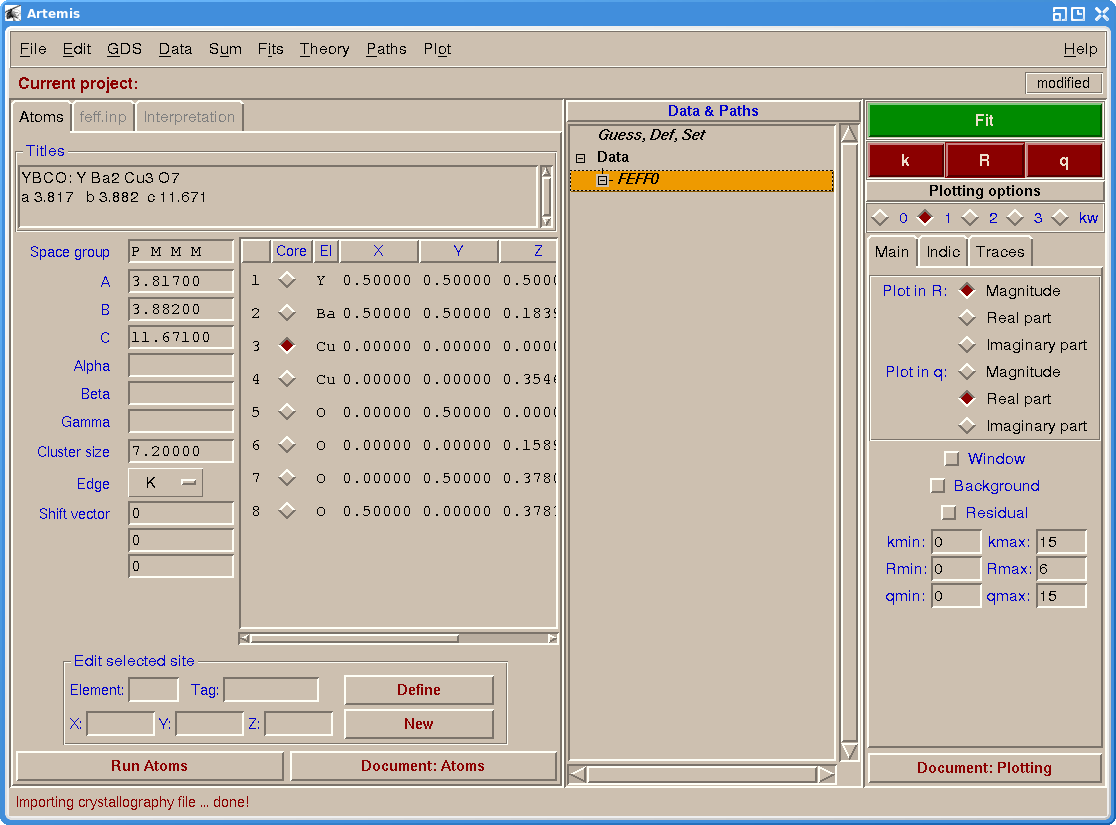
\includegraphics[width=0.7\linewidth]{images/artemis_atoms}
      \end{center}
    \end{column}
    %%
    \begin{column}[c]{0.5\linewidth}
      The input data can be a CIF file or this simple format:
      \begin{block}{}
        \begin{alltt}
          \tiny
 {\color{Green4}title Cobalt sulfide}
 {\color{Green4}title Elliot (1960) J.Chem. Phys. 33(3), 903.}
 {\color{Brown4}space} P a 3
 {\color{Brown4}rmax}=6.0   {\color{Brown4}a}=5.523
 {\color{Brown4}core}=Co
 {\color{Brown4}atoms}
 {\color{Blue4}! At.type   x     y     z      tag}
    Co     0.00000   0.00000   0.00000  Co
    S      0.38900   0.38900   0.38900  S
         \end{alltt}
       \end{block}
     \end{column}
   \end{columns}

   \bigskip

   These data are typically taken from the crystallography literature,
   the \textit{Inorganic Crystal Structure Database}, or from:
   \href{http://cars9.uchicago.edu/\char126newville/adb/search.html}
   {\color{Blue4}\texttt{http://cars9.uchicago.edu/\char126newville/adb/search.html}}
\end{frame}

\begin{frame}[fragile]
  \frametitle{Feff input files for non-crystalline materials}
  \begin{columns}[c]
    \begin{column}{0.6\linewidth}
      There are many sources of structural data about molecules,
      proteins, and other non-crystalline materials. A bit of googling
      turned up this Protein Data Bank File for cisplatin:

      \centering\includegraphics<1>[width=0.4\linewidth]{images/cisplatin}
      \begin{alltt}
        \tiny
ATOM   1 PT1  MOL A  1  -0.142   0.141   7.747  1.00  1.00
ATOM   2 CL2  MOL A  1  -0.135  -2.042   8.092  1.00  1.00
ATOM   3 CL3  MOL A  1   2.064   0.127   7.615  1.00  1.00
ATOM   4  N4  MOL A  1  -0.147   2.166   7.427  1.00  1.00
ATOM   5  N5  MOL A  1  -2.188   0.154   7.870  1.00  1.00
ATOM   6 1H4  MOL A  1   0.793   2.489   7.319  1.00  1.00
ATOM   7 2H4  MOL A  1  -0.570   2.625   8.208  1.00  1.00
ATOM   8 3H4  MOL A  1  -0.668   2.370   6.598  1.00  1.00
ATOM   9 1H5  MOL A  1  -2.464   0.303   8.819  1.00  1.00
ATOM  10 2H5  MOL A  1  -2.546  -0.724   7.552  1.00  1.00
ATOM  11 3H5  MOL A  1  -2.551   0.889   7.298  1.00  1.00
TER
      \end{alltt}
    \end{column}
    %%
    \begin{column}{0.4\linewidth}
      Cut, paste, insert some boilerplate, and voil\'a!
      \begin{block}{}
        \begin{alltt}
          \tiny
 {\color{Green4}TITLE cisplatin}
 {\color{Purple2}HOLE}  4  1.0
 {\color{Purple2}RMAX}  8
 {\color{Brown4}POTENTIALS}
     0   78   Pt
     1   17   Cl
     2    7   N
     3    1   H

 {\color{Brown4}ATOMS}
   -0.142   0.141   7.747   0
   -0.135  -2.042   8.092   1
    2.064   0.127   7.615   1
   -0.147   2.166   7.427   2
   -2.188   0.154   7.870   2
    0.793   2.489   7.319   3
   -0.570   2.625   8.208   3
   -0.668   2.370   6.598   3
   -2.464   0.303   8.819   3
   -2.546  -0.724   7.552   3
   -2.551   0.889   7.298   3
         \end{alltt}
       \end{block}

       ~\\[-5ex]

       {\scriptsize Note that the absorber need not be at
         (0,0,0) and the list need not be in any particular order.}

    \end{column}
  \end{columns}
\end{frame}


%\subsection[Atoms and paths]{Atoms and paths}
%
\begin{frame}
  \frametitle<1>{FeS$_2$: Single scattering paths in a crystal}
  \frametitle<2>{FeS$_2$: Multiple scattering paths in a crystal}
  \begin{columns}[T]
    \begin{column}{0.6\linewidth}
      \begin{center}
        \includegraphics<1>[width=0.6\linewidth]{images/FeS2/fes2}
        \includegraphics<2>[width=0.9\linewidth]{images/FeS2/intrp}
      \end{center}

      \begin{onlyenv}<1>
        \small
        {\color{Chocolate3}$\bullet$} = Fe \quad%
        {\color{Gold2}$\bullet$} = S

        The first sulfur SS path is from the octahedron surrounding
        the Fe atom.  It provides most of the spectral weight under
        the first peak.

        The next two S and one Fe SS paths overlap between 2.5 and
        3.5\,\AA.
      \end{onlyenv}
      \begin{onlyenv}<2>
        \small
        The relationship between the EXAFS spectrum and atomic
        structure can be quite complicated due to multiple
        scattering.

        S--S and S--Fe triangles contribute
        significantly between 2.5 and 3.5\,\AA.
      \end{onlyenv}
    \end{column}
    %%
    \begin{column}{0.4\linewidth}
      \includegraphics<1>[width=\linewidth]{images/FeS2/fourss}
      \includegraphics<2>[width=\linewidth]{images/FeS2/fourms}

      \bigskip

      \includegraphics<1>[width=\linewidth]{images/FeS2/fourss_re}
      \includegraphics<2>[width=\linewidth]{images/FeS2/fourms_re}

      \bigskip

      ~

      \bigskip
    \end{column}
  \end{columns}
  \begin{textblock*}{0.5\linewidth}(0pt,20\TPVertModule) 
    \tiny
    Data from
    \href{http://cars9.uchicago.edu/~newville/ModelLib}
    {\color{Purple4}\texttt{http://cars9.uchicago.edu/~newville/ModelLib}}
  \end{textblock*}
\end{frame}

\begin{frame}
  \frametitle{[Ni(CN)$_4$]$^{2-}$: Paths in a molecule}
  \begin{columns}
    \begin{column}{6cm}
      \begin{center}
        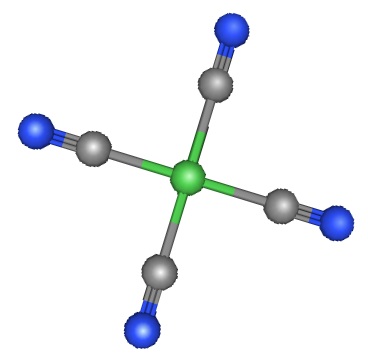
\includegraphics[width=3cm]{images/NiCN/nicn}

        {\color{Green4}$\bullet$} = Ni\quad
        {\color{Gray0}$\bullet$} = C\quad
        {\color{Blue2}$\bullet$} = N
      \end{center}
      Multiple scattering is \textbf{not} just for the materials
      scientists.  [Ni(CN)$_4$]$^{2-}$ in solution is \textbf{not} a
      crystal.

      Without consideration of the MS paths, the huge second peak in
      these data cannot be fit.
    \end{column}
    %%
    \begin{column}{4cm}
      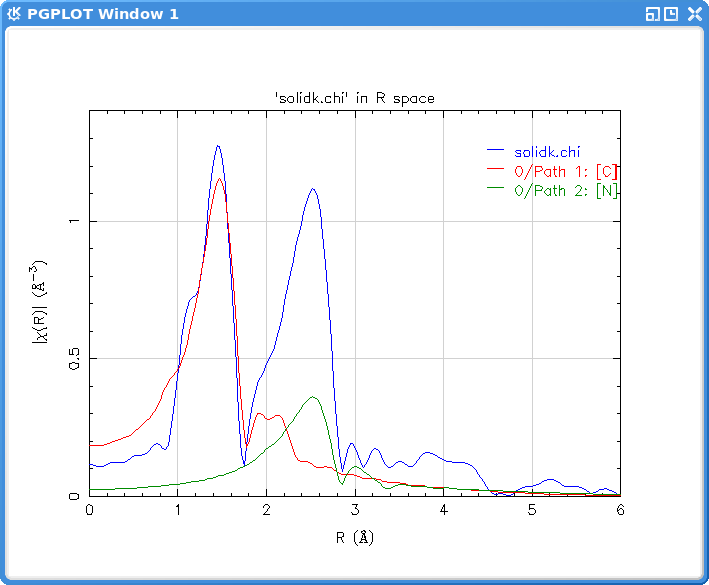
\includegraphics[width=\linewidth]{images/NiCN/ss}

      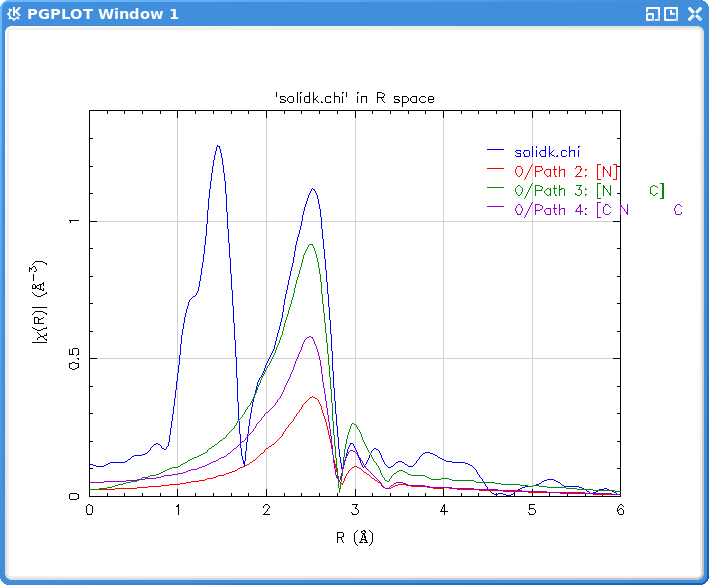
\includegraphics[width=\linewidth]{images/NiCN/ms}
    \end{column}
  \end{columns}
  \begin{textblock*}{0.5\linewidth}(0pt,20\TPVertModule) 
    \tiny
    A.\ Mu\~noz-P\'aez et al. Inorg.\ Chem. \textbf{39} (2000) pp.\ 3784--3790
  \end{textblock*}
\end{frame}

%%% Local Variables:
%%% mode: latex
%%% TeX-master: "pimst2"
%%% End:

%\subsection[Good practice]{Using \textsc{feff} well}
%\begin{frame}[fragile]
  \frametitle{Starting from analogs}
  \begin{columns}[T]
    \begin{column}{0.5\linewidth}
      \begin{center}
        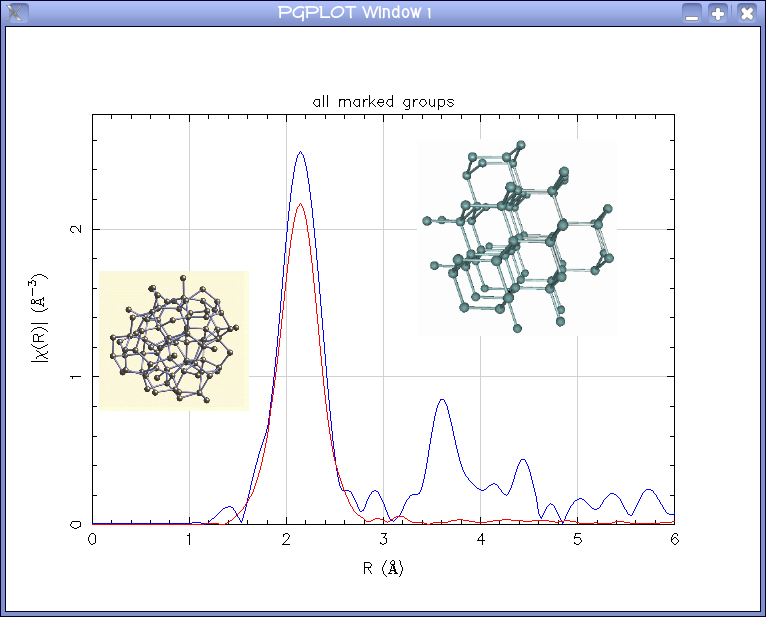
\includegraphics[width=0.9\linewidth]{images/ge_chir_bns}
      \end{center}

      \bigskip

      Use the \texttt{`feff0001.dat'} file from the Ge
      crystal \textsc{feff} calculation

    \end{column}
    \begin{column}{0.5\linewidth}
      \begin{block}{}
        \begin{alltt}
          \tiny
 {\color{Green4}title germanium diamond structure}
 {\color{Brown4}space} f d 3 m
 {\color{Brown4}rmax}=6.0   {\color{Brown4}a}=5.658
 {\color{Brown4}atoms}
 {\color{Blue4}! At.type   x     y     z      tag}
    Ge      1/8   1/8   1/8
         \end{alltt}
       \end{block}

       \begin{center}
         \scriptsize
         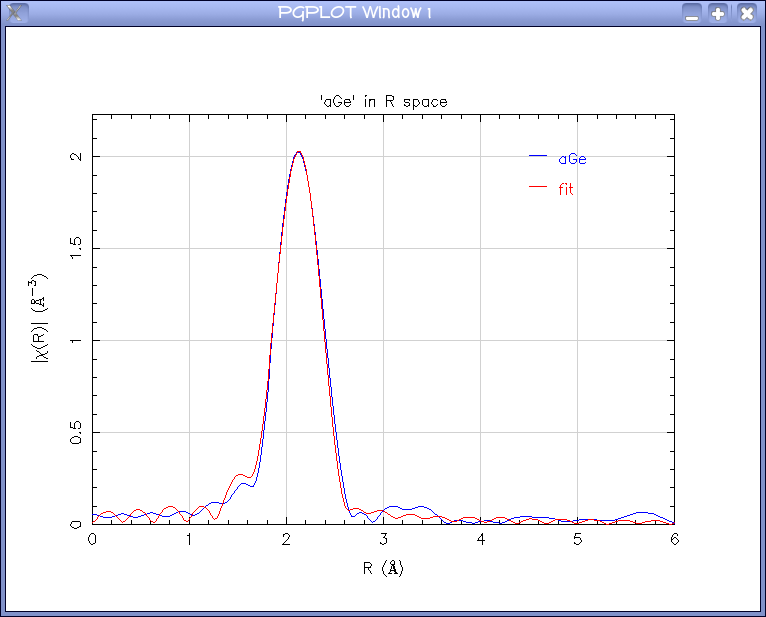
\includegraphics[width=0.85\linewidth]{images/ge_fit}

         \medskip

         \begin{tabular}{lcc}
           & crystal & amorphous \\
           \hline
           N & 4 & 4.0(8) \\
           $R_1$ (\AA) & 2.441(3) & 2.451(11) \\
           $\sigma^2$ (\AA$^2$) & 0.00419(55) & 0.00528(155) \\
         \end{tabular}
       \end{center}
    \end{column}
  \end{columns}
  \begin{textblock*}{0.5\linewidth}(0pt,19\TPVertModule) \tiny
    Crystalline data is from the 
    \href{http://www.nsls.bnl.gov/beamlines/x18b/data.htm}
    {\color{Purple4}NSLS X18 standards database}.
    Amorphous data courteously provided by Dale Brewe and Joe Woicik.
  \end{textblock*}
\end{frame}

\begin{frame}[fragile]
  \frametitle{Close is usually good enough}
  \begin{columns}[T]
    \begin{column}{0.5\linewidth}
      Solid solution of AgBr$_{0.5}$Cl$_{0.5}$ at 20\,K

      \bigskip

      The first shell contains both Br and Cl scatterers.  We use the
      known crystal structure for AgBr to compute the Ag--Br path.
      \begin{block}{}
        \begin{alltt}
          \tiny
 {\color{Green4}title rocksalt silver bromide at room temperature}
 {\color{Brown4}space} F M -3 M
 {\color{Brown4}rmax}=6   {\color{Brown4}a}=5.7745
 {\color{Brown4}core}=Ag
 {\color{Brown4}atoms}
 {\color{Blue4}! At.type   x     y     z      tag}
    Ag      0.0   0.0   0.0
    Br      1/2   1/2   1/2
         \end{alltt}
       \end{block}
       We simply replace Br with Cl and run \textsc{atoms} and
       \textsc{feff} again.
    \end{column}
    %%
    \begin{column}{0.5\linewidth}
      \begin{center}
        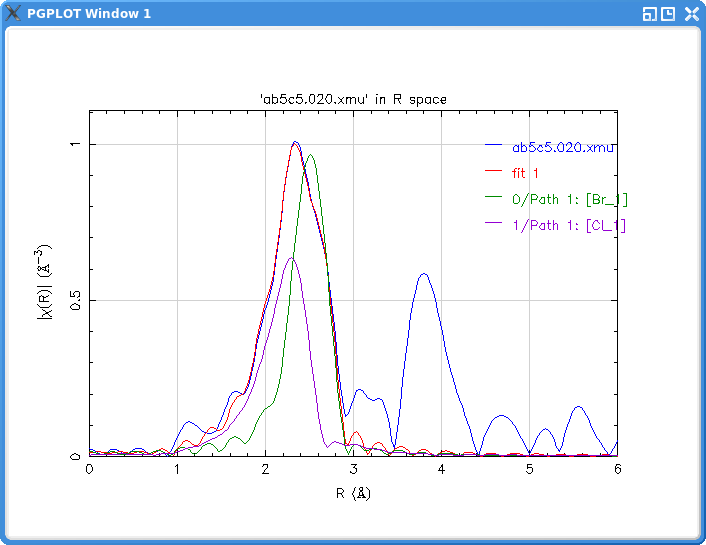
\includegraphics[width=0.9\linewidth]{images/abcfit}

        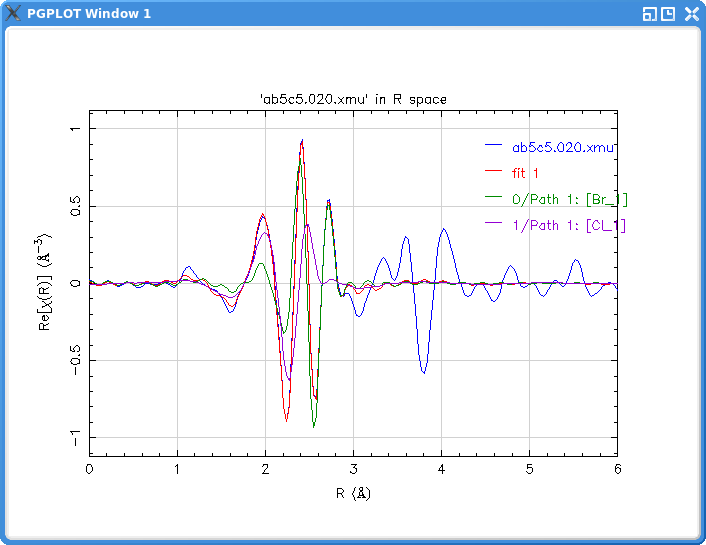
\includegraphics[width=0.9\linewidth]{images/abcfit_re}
      \end{center}

    \end{column}
  \end{columns}

  \medskip

  \begin{center}
    %%\scriptsize{
    $\Delta R_\mathrm{Br}=-0.032(4)\mathrm{\AA}$ \qquad
    {\color{Red3}$\Delta R_\mathrm{Cl}=-0.105(12)\mathrm{\AA}$}
    %%$\sigma^2_\mathrm{Br}=0.00499(41)\mathrm{\AA}^2$,
    %%$\sigma^2_\mathrm{Cl}=0.00719(165)\mathrm{\AA}^2$,
    %%}
  \end{center}
\end{frame}

\begin{frame}
  \frametitle{Pick and choose}
  \begin{columns}
    \begin{column}{0.5\linewidth}
      The data are uranyl acetate mixed with a \textit{B. Subtilis}
      culture and brought to equilibrium at $\mathrm{pH}\sim8$.

      \begin{center}
        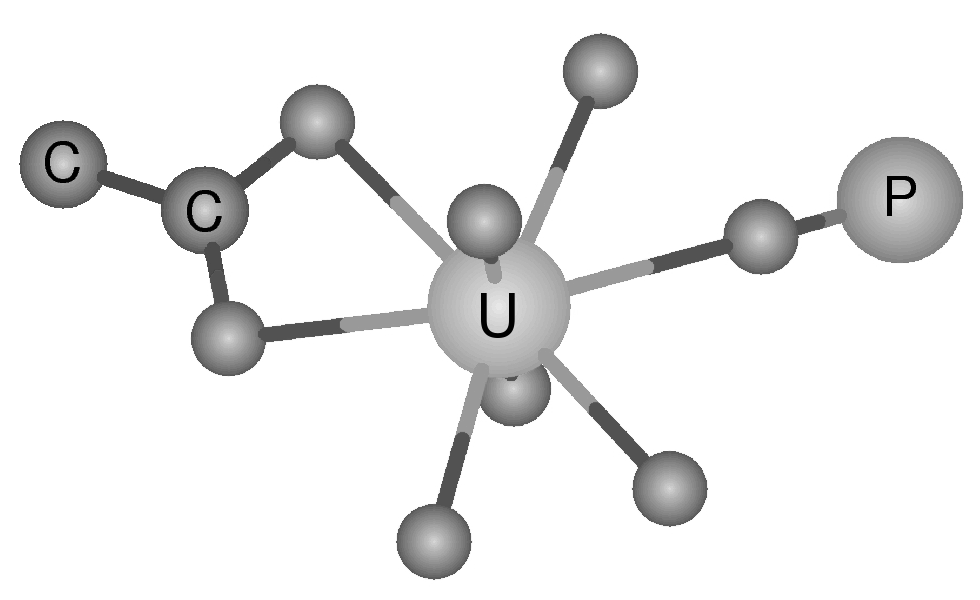
\includegraphics[width=3cm]{images/UPC_bw}
      \end{center}
    \end{column}
    %%%
    \begin{column}{0.5\linewidth}
      \centering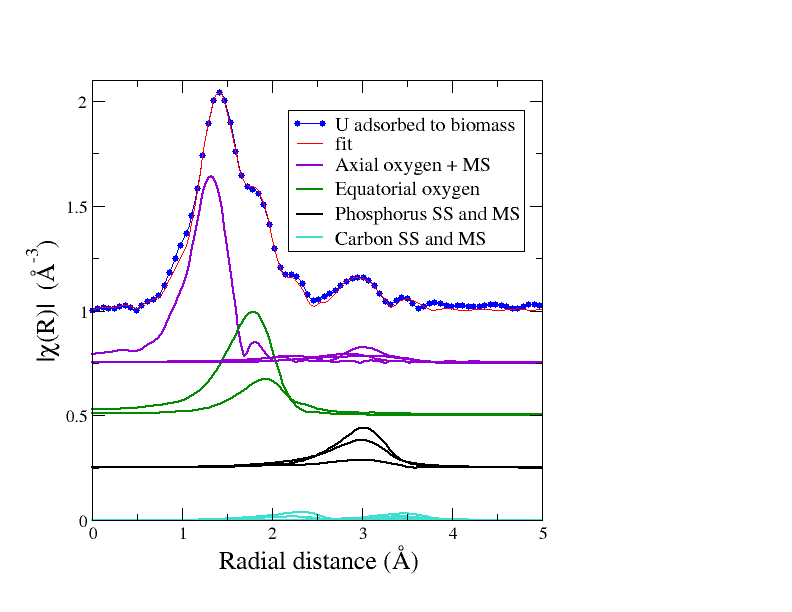
\includegraphics[width=\linewidth]{images/ubs}
    \end{column}
  \end{columns}
  \begin{description}
  \item[triuranyl diphoshate tetrahydrate] This mineral provides paths
    for axial and equatorial O of the appropriate lengths as well as
    SS and MS to the monodentate P
  \item[Rutherfordine, UO$_2$CO$_3$] This mineral provides paths for
    SS and MS involving the bidentate C
  \end{description}
  \begin{textblock*}{0.5\linewidth}(0pt,20\TPVertModule) \tiny S.D.\
    Kelly \textit{et al}., Geochimica et Cosmochimica Acta,
    \textbf{66}:22, pp.\ 3855–-3871, 2002
  \end{textblock*}



\end{frame}

%%% Local Variables:
%%% mode: latex
%%% TeX-master: "pimst2"
%%% End:


\begin{frame}
  \frametitle{Multiple scattering and EXAFS: FeS$_2$}
  \begin{columns}
    \begin{column}{0.5\linewidth}
      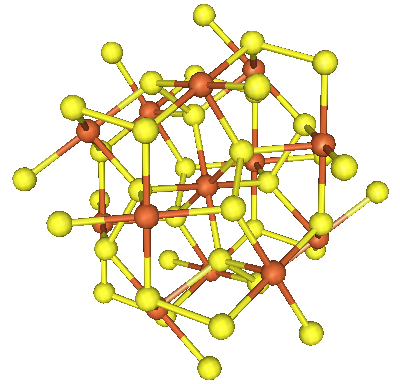
\includegraphics[width=\linewidth]{images/FeS2/fes2.png}
      \begin{center}
        {\color{Chocolate3}$\bullet$} = Fe \quad%
        {\color{Gold2}$\bullet$} = S
      \end{center}
    \end{column}
    \begin{column}{0.5\linewidth}
      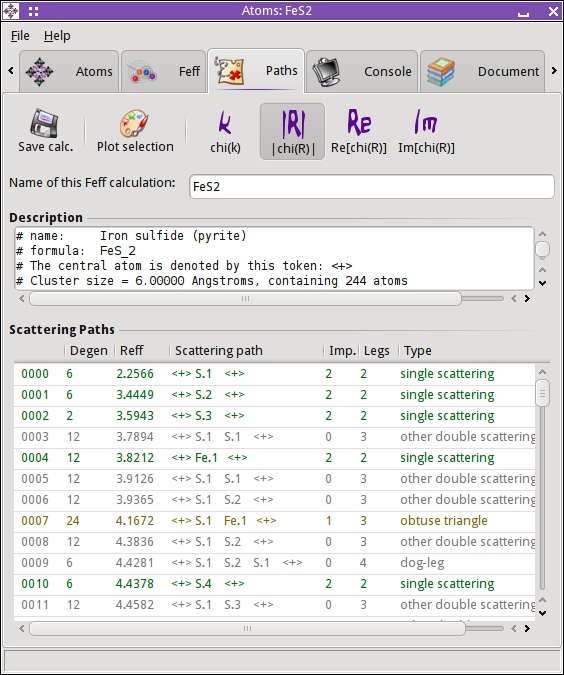
\includegraphics[width=\linewidth]{images/intrp.png}
    \end{column}
  \end{columns}
\end{frame}

\begin{frame}
  \frametitle{Multiple scattering and EXAFS: SS}
  \begin{columns}
    \begin{column}{0.5\linewidth}
      The first sulfur SS path is from the octahedron surrounding the
      Fe atom.  It provides most of the spectral weight under the
      first peak.

      \medskip

      The next two S and one Fe SS paths overlap between 2.5 and
      3.5\,\AA.
    \end{column}
    \begin{column}{0.5\linewidth}
      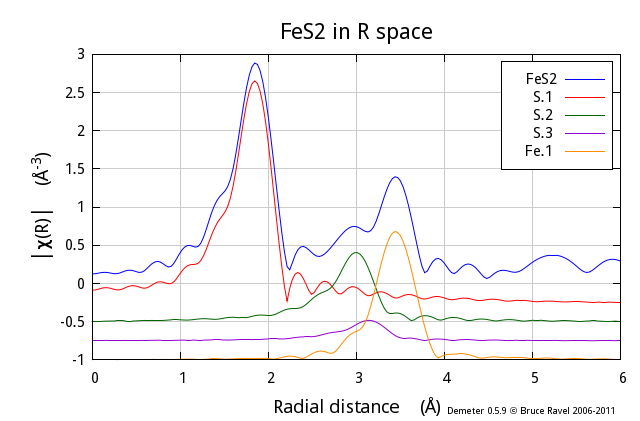
\includegraphics[width=\linewidth]{images/fes2_ss.png}
    \end{column}
  \end{columns}
\end{frame}

\begin{frame}
  \frametitle{Multiple scattering and EXAFS: MS}
  \begin{columns}
    \begin{column}{0.5\linewidth}
      The relationship between the EXAFS spectrum and atomic
      structure can be quite complicated due to multiple
      scattering.

      \medskip

      S--S and S--Fe triangles contribute
      significantly between 2.5 and 3.5\,\AA.

      \medskip

      Collinear paths through the absorber involving 1$^{st}$ shell S
      atoms contribute significantly around 3.9\,\AA.
    \end{column}
    \begin{column}{0.5\linewidth}
      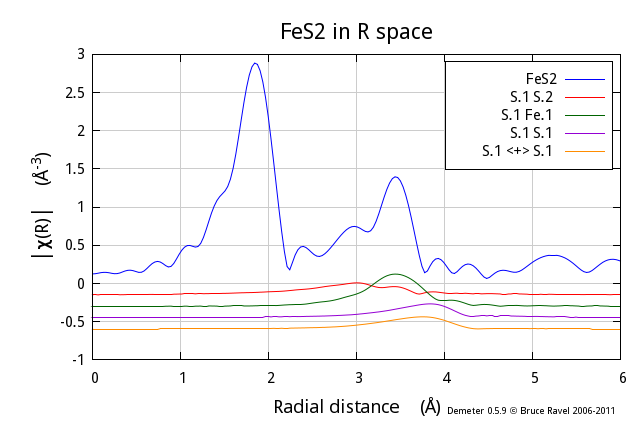
\includegraphics[width=\linewidth]{images/fes2_ms.png}
    \end{column}
  \end{columns}
\end{frame}

\section[Resources]{Resources}

\begin{frame}
  \frametitle{Resources}
  \begin{itemize}
  \item Websites
    \begin{itemize}
    \item \footnotesize
      \href{http://xafs.org}{\color{Blue4}\texttt{http://xafs.org}}
      offers tutorials, links to resources, information about upcoming
      workshops, and much more
    \item \textsc{ifeffit} homepage:
      \href{http://cars9.uchicago.edu/iffwiki/About}
      {\color{Blue4}\texttt{http://cars9.uchicago.edu/iffwiki/About}}
    \item \textsc{feff} homepage:
      \href{http://feff.phys.washington.edu}
      {\color{Blue4}\texttt{http://feff.phys.washington.edu}}
    \item \textsc{athena} and \textsc{artemis}:
      \href{http://github.com/bruceravel/demeter}
      {\color{Blue4}\texttt{http://github.com/bruceravel/demeter/}}
    \end{itemize}
  \item Journal articles
    \begin{itemize}
    \item \footnotesize The \textsc{feff} reference: Rehr and Albers review article:   J.J.~Rehr and R.C.~Albers,
      Rev.\ Mod.\ Phys.\ \textbf{72}:3 (2000) pp.\ 621--654
    \item Two excellent references on multiple scattering theory:
      J.L.~Beeby, Proc.\ Royal Soc.\ \textbf{A274} (1964) pp.\
      309--317 and \textbf{A279} (1967) pp.\ 82--97.
    \end{itemize}
  \item Other Software
    \begin{itemize}
    \item \footnotesize XANES calculations using Mulitplets:
      \href{http://xafs.org/Software/TtMultiplet}
      {\color{Blue4}\texttt{http://xafs.org/Software/TtMultiplet}}
    \item XANES calculations by finite difference method:
      \href{http://xafs.org/Software/FDMNES}
      {\color{Blue4}\texttt{http://xafs.org/Software/FDMNES}}
    \item Band structure: The work of Eric Shirley
      (\href{http://physics.nist.gov/Divisions/Div844/facilities/theorModel/tmopm.html}
      {\color{Blue4}\tiny \texttt{http://physics.nist.gov/Divisions/Div844/facilities/theorModel/tmopm.html}}) and
      Aleksi Soininen, Helsinki University
    \item XANES fitting: \textsc{FitIt} (\href{http://xafs.org/Software/FitIt}{\color{Blue4}\texttt{http://xafs.org/Software/FitIt}})
      and \textsc{mxan} (PRB \textbf{65} (2002) 174205).
    \end{itemize}
  \end{itemize}
\end{frame}


\end{document}


%%% Local Variables:
%%% TeX-parse-self: t
%%% TeX-auto-save: t
%%% TeX-auto-untabify: t
%%% TeX-PDF-mode: t
%%% End:
